\newpage
\section{Punto 4}
\textit{A partir del primer árbol B de la figura \ref{fig:Arbol1}, dibujar el árbol resultante, luego de insertar consecutivamente los
elementos 30 y 32.
}\\
\begin{figure}
  \centering
  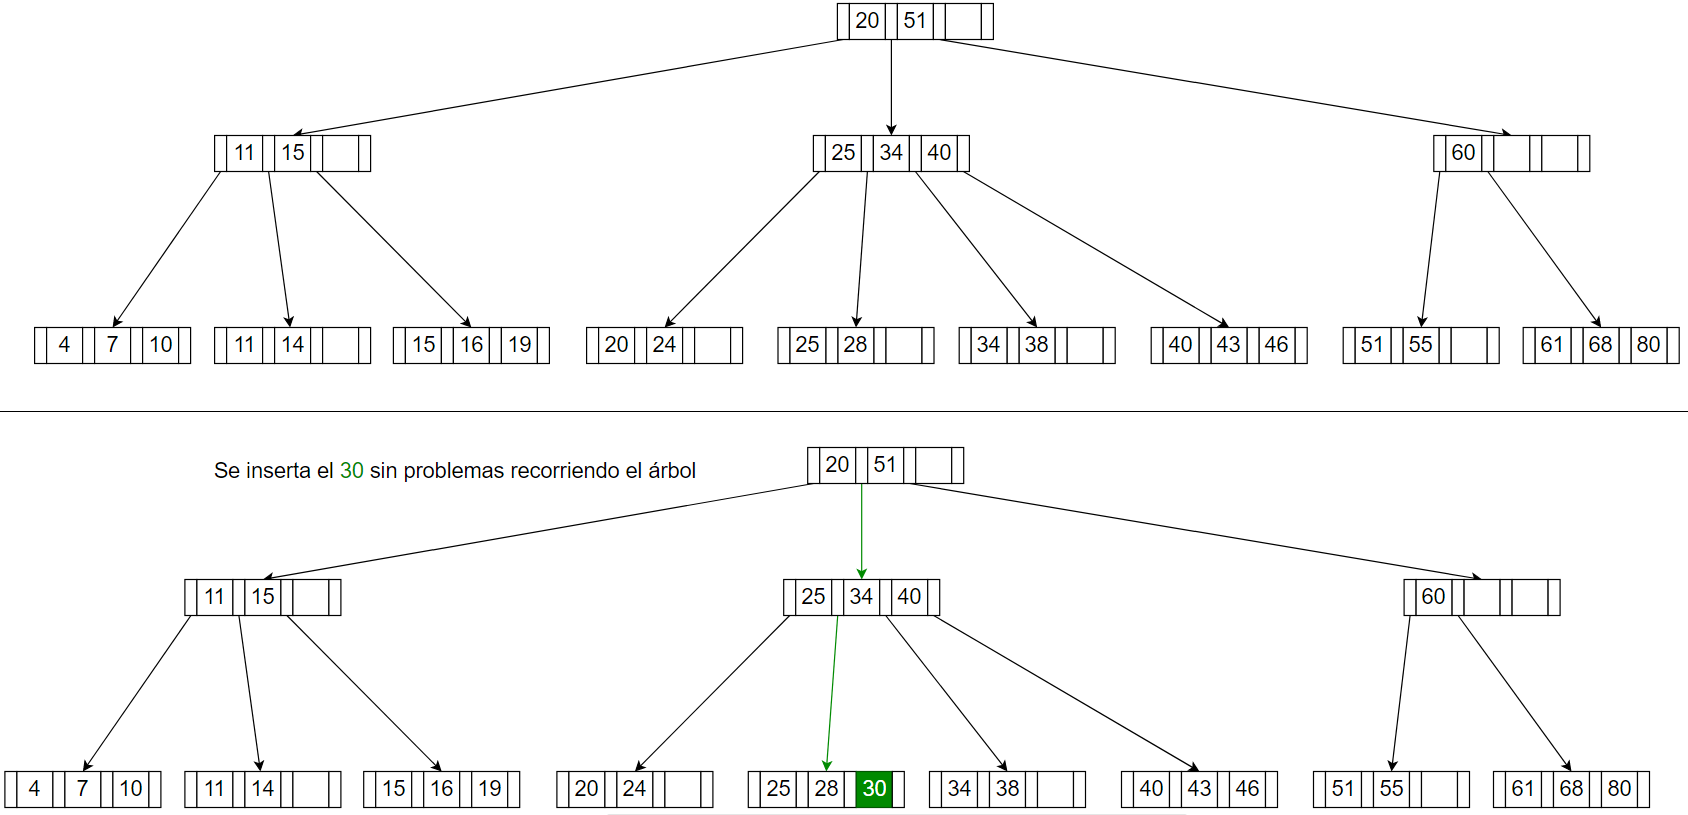
\includegraphics[width=\textwidth, scale=1]{Images/Punto4/Arbol1.png}
  \caption{Inserción de los elementos 30 y 32 de manera consecutiva en árbol B \textbf{(imagen en alta resolución en \cite{arbolB})}}
  \label{fig:Arbol1}
\end{figure}

\begin{figure}
  \centering
  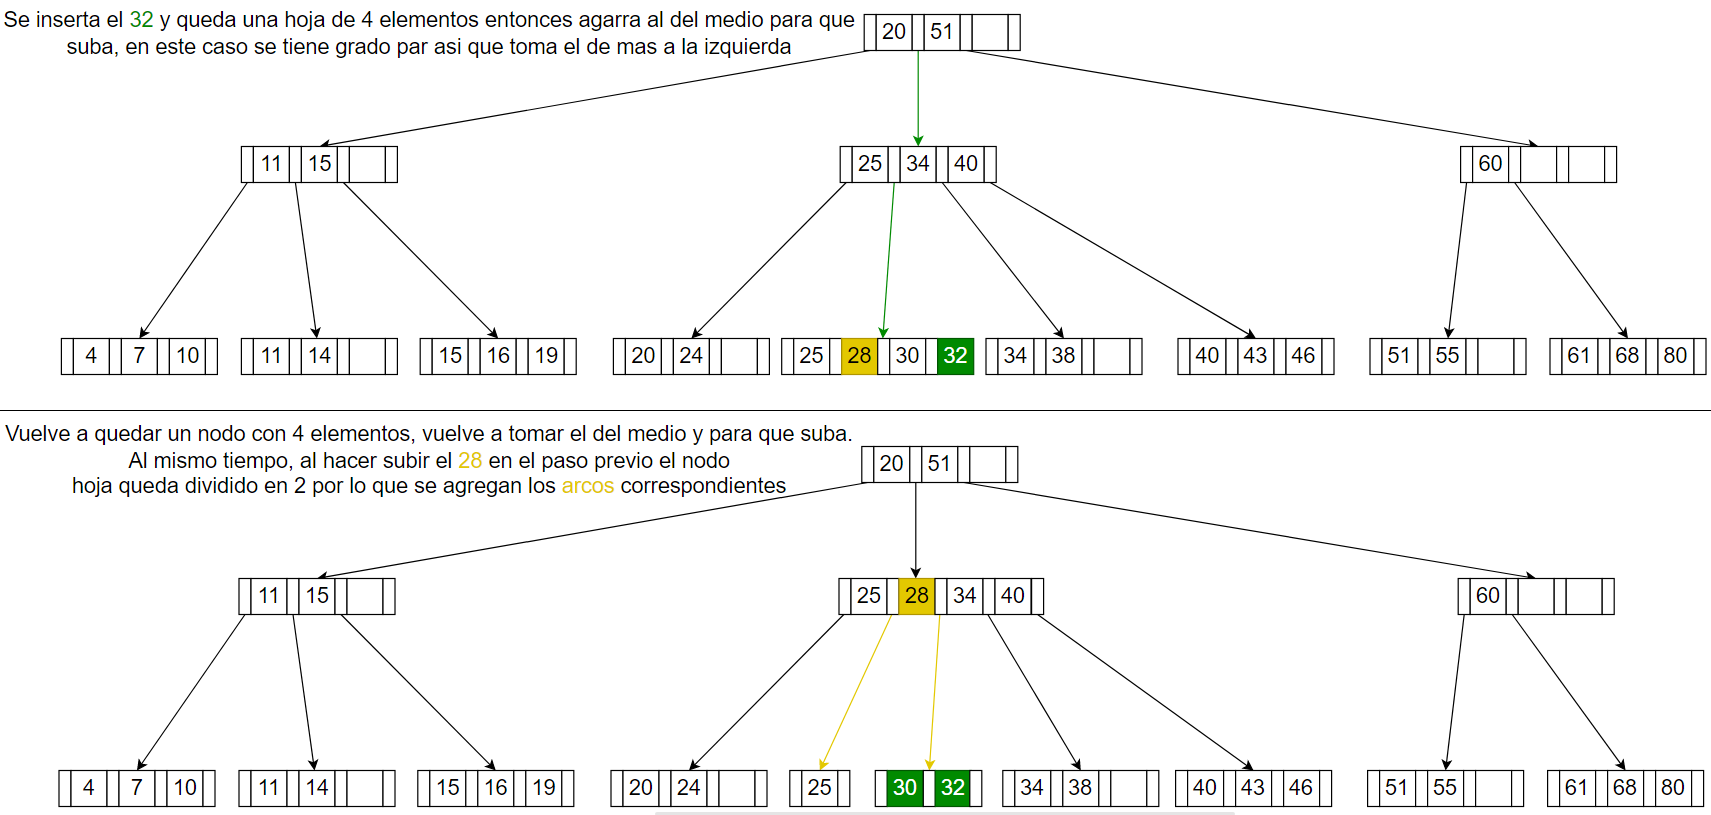
\includegraphics[width=\textwidth, scale=1]{Images/Punto4/Arbol2.png}
  \caption{Inserción de los elementos 30 y 32 de manera consecutiva en árbol B \textbf{(imagen en alta resolución en \cite{arbolB})}}
  \label{fig:Arbol2}
\end{figure}

\begin{figure}
  \centering
  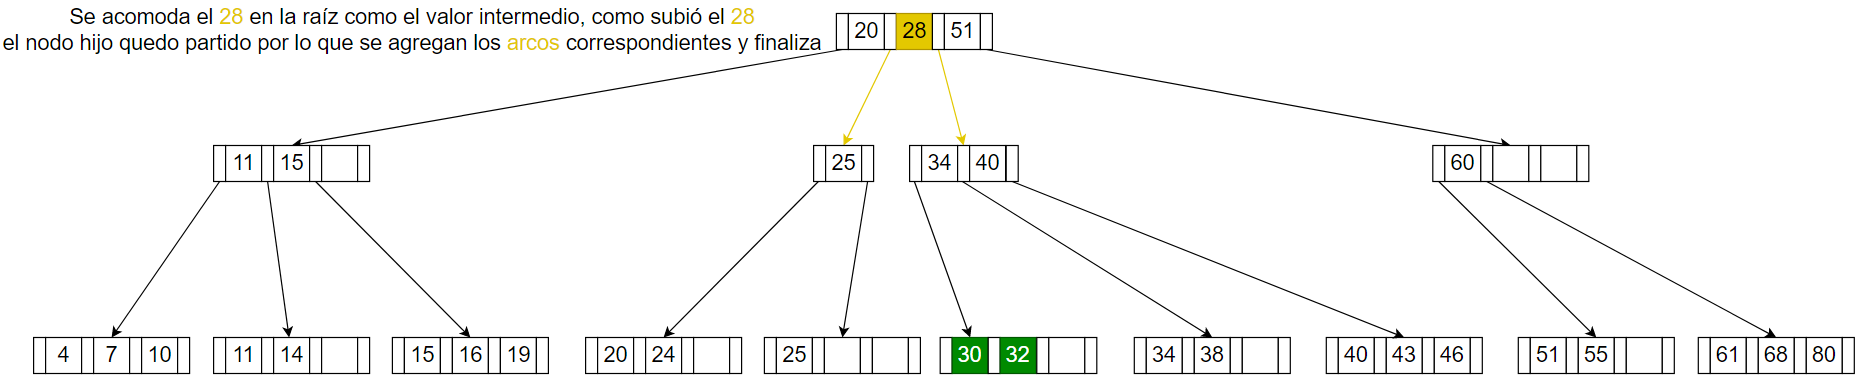
\includegraphics[width=\textwidth, scale=1]{Images/Punto4/Arbol3.png}
  \caption{Inserción de los elementos 30 y 32 de manera consecutiva en árbol B \textbf{(imagen en alta resolución en \cite{arbolB})}}
  \label{fig:Arbol3}
\end{figure}
